\documentclass[11pt, twoside]{memoir}

\setsecnumdepth{subsubsection}
\settocdepth{subsubsection}

\usepackage[normalem]{ulem}

\usepackage{fontspec}
	\setmainfont%
		[Mapping=tex-text]
	{Cambria}
	\setsansfont%
%	[Ligatures={NoCommon, NoDiscretionary},%
		[Mapping=tex-text]%
		{Inconsolata}
\usepackage{relsize}

\def\textlabel#1{{\relsize{-.5}\fontspec[Mapping=tex-text]{Roboto Mono}{#1}}}
\def\langtext#1{\textit{#1}}

\usepackage{float}

\usepackage[top=1in, bottom=1in, left=1.25in, right=1.25in]{geometry}

\usepackage{xcolor}

\usepackage{hyperref}

\renewcommand\cftappendixname{\appendixname~}
\usepackage[nonumberlist, nopostdot, section=chapter, numberedsection=autolabel]{glossaries}
\makeglossaries

\usepackage{tikz}
\usetikzlibrary{shapes, arrows, backgrounds, fit, positioning}
\usetikzlibrary{decorations.pathreplacing}
\tikzset{
    dots/.style={
        line width=4pt,
        line cap=round,
        dash pattern=on 0pt off 6pt
    }
}
\usepackage{colortbl}
	\definecolor{CB1}{RGB}{0, 114, 178}%BLUE
	\definecolor{CB2}{RGB}{213, 94, 0}%VERMILLION
	\definecolor{CB3}{RGB}{0, 158, 115}%BLUE GREEN
	\definecolor{CB4}{RGB}{204, 121, 167}%REDDISH PURPLE
	\definecolor{CB5}{RGB}{86, 180, 233}%SKY BLUE
	\definecolor{CB6}{RGB}{230, 159, 0}%ORANGE
	\definecolor{CB7}{RGB}{240, 228, 66}%YELLOW
	\def\CB#1#2{\textcolor{CB#1}{#2}}
\usepackage{booktabs, longtable, array, arydshln, multirow}
\usepackage{caption}
\newlength\defaultaboverulesep
\setlength\defaultaboverulesep{\aboverulesep}
\newlength\defaultbelowrulesep
\setlength\defaultbelowrulesep{\belowrulesep}
\setlength\aboverulesep{0pt}
\setlength\belowrulesep{0pt}
\def\arraystretch{1.15}

\usepackage[framemethod=tikz]{mdframed}
	\newmdenv[middlelinecolor=CB1,
		middlelinewidth=1pt,
		backgroundcolor=gray!50,
		roundcorner=4pt]{infobox}
	\newmdenv[middlelinecolor=CB2,
		middlelinewidth=2pt,
		backgroundcolor=CB2!30,
		roundcorner=4pt]{toexpand}

\usepackage{makeidx}
\usepackage{graphicx}
	\graphicspath{{figures}}

\usepackage{expex}

\usepackage{enumitem}
	\setitemize{itemsep=.5ex, topsep=1ex, parsep=0pt, partopsep=0pt, leftmargin=3em, rightmargin=0ex}
	\setenumerate{itemsep=.5ex, topsep=1ex, parsep=0pt, partopsep=0pt, leftmargin=3em, rightmargin=0em}
\usepackage[hang, flushmargin, multiple, bottom, stable]{footmisc}

\usepackage{fancyhdr}

\usepackage{natbib}
	\bibpunct[:]{(}{)}{,}{a}{}{,}
	\setlength{\bibsep}{1ex plus 0.3ex}
\renewcommand{\bibsection}{\part*{Bibliography}}

\usepackage{cite-ref-errors}

\setlength\parskip{.5\baselineskip}
\setlength\parindent{0pt}
\frenchspacing
\raggedbottom

\def\THIStitle{Embarking on PoLaR Explorations}
\def\THISsubtitle{A Framework for Intonational Annotation and Analysis}
\pagestyle{fancy}
	\fancyhead[LO]{\textit{\THIStitle}}
	\fancyhead[RO]{}
	\fancyhead[LE]{}
	\fancyhead[RE]{Ahn, Veilleux, Shattuck-Hufnagel, Brugos}
\pagestyle{plain}
\hypersetup{
	breaklinks=true,
	pdfauthor={Byron Ahn, Nanette Veilleux, Stefanie Shattuck-Hufnagel, and Alejna Brugos},
	pdftitle={\THIStitle: \THISsubtitle},
	bookmarks,
	bookmarksopen=true,
	colorlinks=false,
	allcolors=blue
}

\makeindex

\begin{document}
\frontmatter
\captionsetup{margin=1.5cm, skip=4pt, labelfont={bf, footnotesize}, textfont={footnotesize}}

\title{\THIStitle}
\author{Byron Ahn \and Nanette Veilleux \and Stefanie Shattuck-Hufnagel \and Alejna Brugos}
\date{\today}
%{\normalsize\textcolor{red}{These guidelines are still under active development.\\Find the latest version of the guidelines, as well as .wav files, .TextGrid files, and some scripts, at \url{https://www.polarlabels.com/}.}}

\begin{titlingpage}
\vspace*{\fill}
\begin{center}
\textbf{\huge{\THIStitle:\strut}}\\
\textbf{\huge{\THISsubtitle\strut}}
\\[6\baselineskip]
{\large{Byron Ahn,\strut\\Nanette Veilleux,\strut\\Stefanie Shattuck-Hufnagel,\strut\\and Alejna Brugos\strut}}\\[6\baselineskip]
{\large\textit{draft}}\\
November 2022
\end{center}
\vspace*{\fill}
\end{titlingpage}

\tableofcontents
\newpage
\listoffigures
\listoftables
\newpage

\mainmatter

\chapter{PoLaR Beyond these Current Guidelines}\label{ch:beyond}
Up to this point, PoLaR labels have been (purposefully) defined in a way that allows them to be used with a variety of phonological analyses. For example, the PrStr tier labels for prominences and boundaries  are not defined according to any particular phonological inventory, but rather encode distinctions that are widely adopted by a variety of theorists and that apply widely across languages and language varieties.

While this reduction in theoretical commitments is useful for ensuring that labels produced by annotators working in a variety of phonological frameworks can be compared, PoLaR labellers may also want to annotate more detail and insight, as informed by other frameworks or theories. PoLaR labelling systematically places all prosodic annotations in one place, which is useful for later analysis, and its extensibility provides the option of adding new labelling options, while ensuring that these additional labels can be easily ignored by other labellers who prefer to do so, and also (critically) by PoLaR-related scripts.

To allow PoLaR users to do this, while preserving PoLaR as a single prosodic annotation system whose labels can be compared across labelling groups, we offer two means of extending PoLaR. First, users can add “tags” to existing PoLaR labelling tiers, that take on a form like \textlabel{\#X}, where X is any parameter of interest, and the \textlabel{\#} symbol identifies the label as a non-core PoLaR annotation. Second, a user can add additional tiers where appropriate. In the remainder of this section, these two methods of extending PoLaR will be illustrated with examples from several different domains. The illustrative labels and tiers introduced in this section are not to be taken as a core aspect of PoLaR. None of them are intended as necessary for PoLaR annotation.

\section{Tagging a Deeper Analysis (Expert-Level Labellers Only)}\label{sec:tagging-a-deeper-analysis-expert-level-labellers-only}

For certain goals and datasets, it may be useful to systematically label more specific analyses. To allow this flexibility, while also remaining consistent to enable comparison across labellers, an ‘analysis tag’ —introduced with a ‘\textlabel{\#}’ delimiter— can be added to an existing PoLaR labelling tier.

\begin{longtable}{cp{.8\linewidth}} \toprule \textbf{Tag} & \textbf{Significance} \tabularnewline
\midrule \endhead
\textlabel{\#X} & The PoLaR label to which this tag has been added is being analyzed as having property X (where X is a variable). \tabularnewline
\bottomrule
\caption[A proposal for a means to encode additional grammatical analyses.]{A proposal for a means to encode additional grammatical analyses. (Note that these \#X tags can be stacked, to create a PrStr label such as \textlabel{]\#X\#Y\#Z}, indicating a perceived boundary that has characteristics X, Y and Z.)}
\end{longtable}

For example, a labeller who would like to distinguish nuclear stress prominences can augment the PrStr \textlabel{*} label to create \textlabel{*\#NS}. Below we discuss several particular cases where we anticipate that such ‘analysis tags’ may be useful.

\subsection{Categories of Prosodic Phrasing}\label{sec:categories-of-prosodic-phrasing}

English has been argued to make reference the following elements prosodic structure, in its intonational phonology:

\begin{longtable*}{p{.85\linewidth}}
\uline{A Prosodic Hierarchy of English} (cf. \citealt{nesporvogel86, shattuck-hufnagel-96, fery17}) \newline
syllable (σ) < foot (Σ / Ft) < word (ω) < phonological phrase (φ) / intermediate phrase (ip) < intonational phrase (ι / IP) < Utterance (υ / Utt) \\
\end{longtable*}

A labeller who adheres to this (or some other) prosodic hierarchy may wish to keep track of particular prosodic boundaries in PoLaR labels, instead of the perceptually (and not phonologically) defined labels like \textlabel{]} (or \textlabel{[}, \textlabel{]]}, and \textlabel{[[}). This can be achieved with analysis tags like \textlabel{\#IP}, to create PrStr annotations like \textlabel{]\#IP}, to indicate the right edge of an intonation phrase.

These sorts of tags may be especially useful for languages that make use of more than two phrasal levels of prosodic hierarchy (e.g., a labeller of Korean may wish to use \textlabel{]\#AP}, \textlabel{]\#ip}, and \textlabel{]\#IP}; see \citealt{jun07}), or for languages\slash varieties\slash data whose prosodic hierarchy is less clear but for which more than two hierarchical elements can be identified. A labeller of such data where the phonological analysis is still uncertain may wish to use labels like \textlabel{]\#A}, \textlabel{]\#B}, \textlabel{]\#C}, etc., to remain agnostic about particular analyses.

Two examples are given below. The first is an example from MAE\_ToBI training materials (se also \citealt{beckman-05}). In this Advanced PoLaR annotation, each \textlabel{]} on the PrStr tier is annotated with MAE\_ToBI’s numerical labels for constituent categories in the prosodic hierarchy: \textlabel{\#2}, \textlabel{\#3}, and \textlabel{\#4}.

\begin{figure}[H]
\centering
%
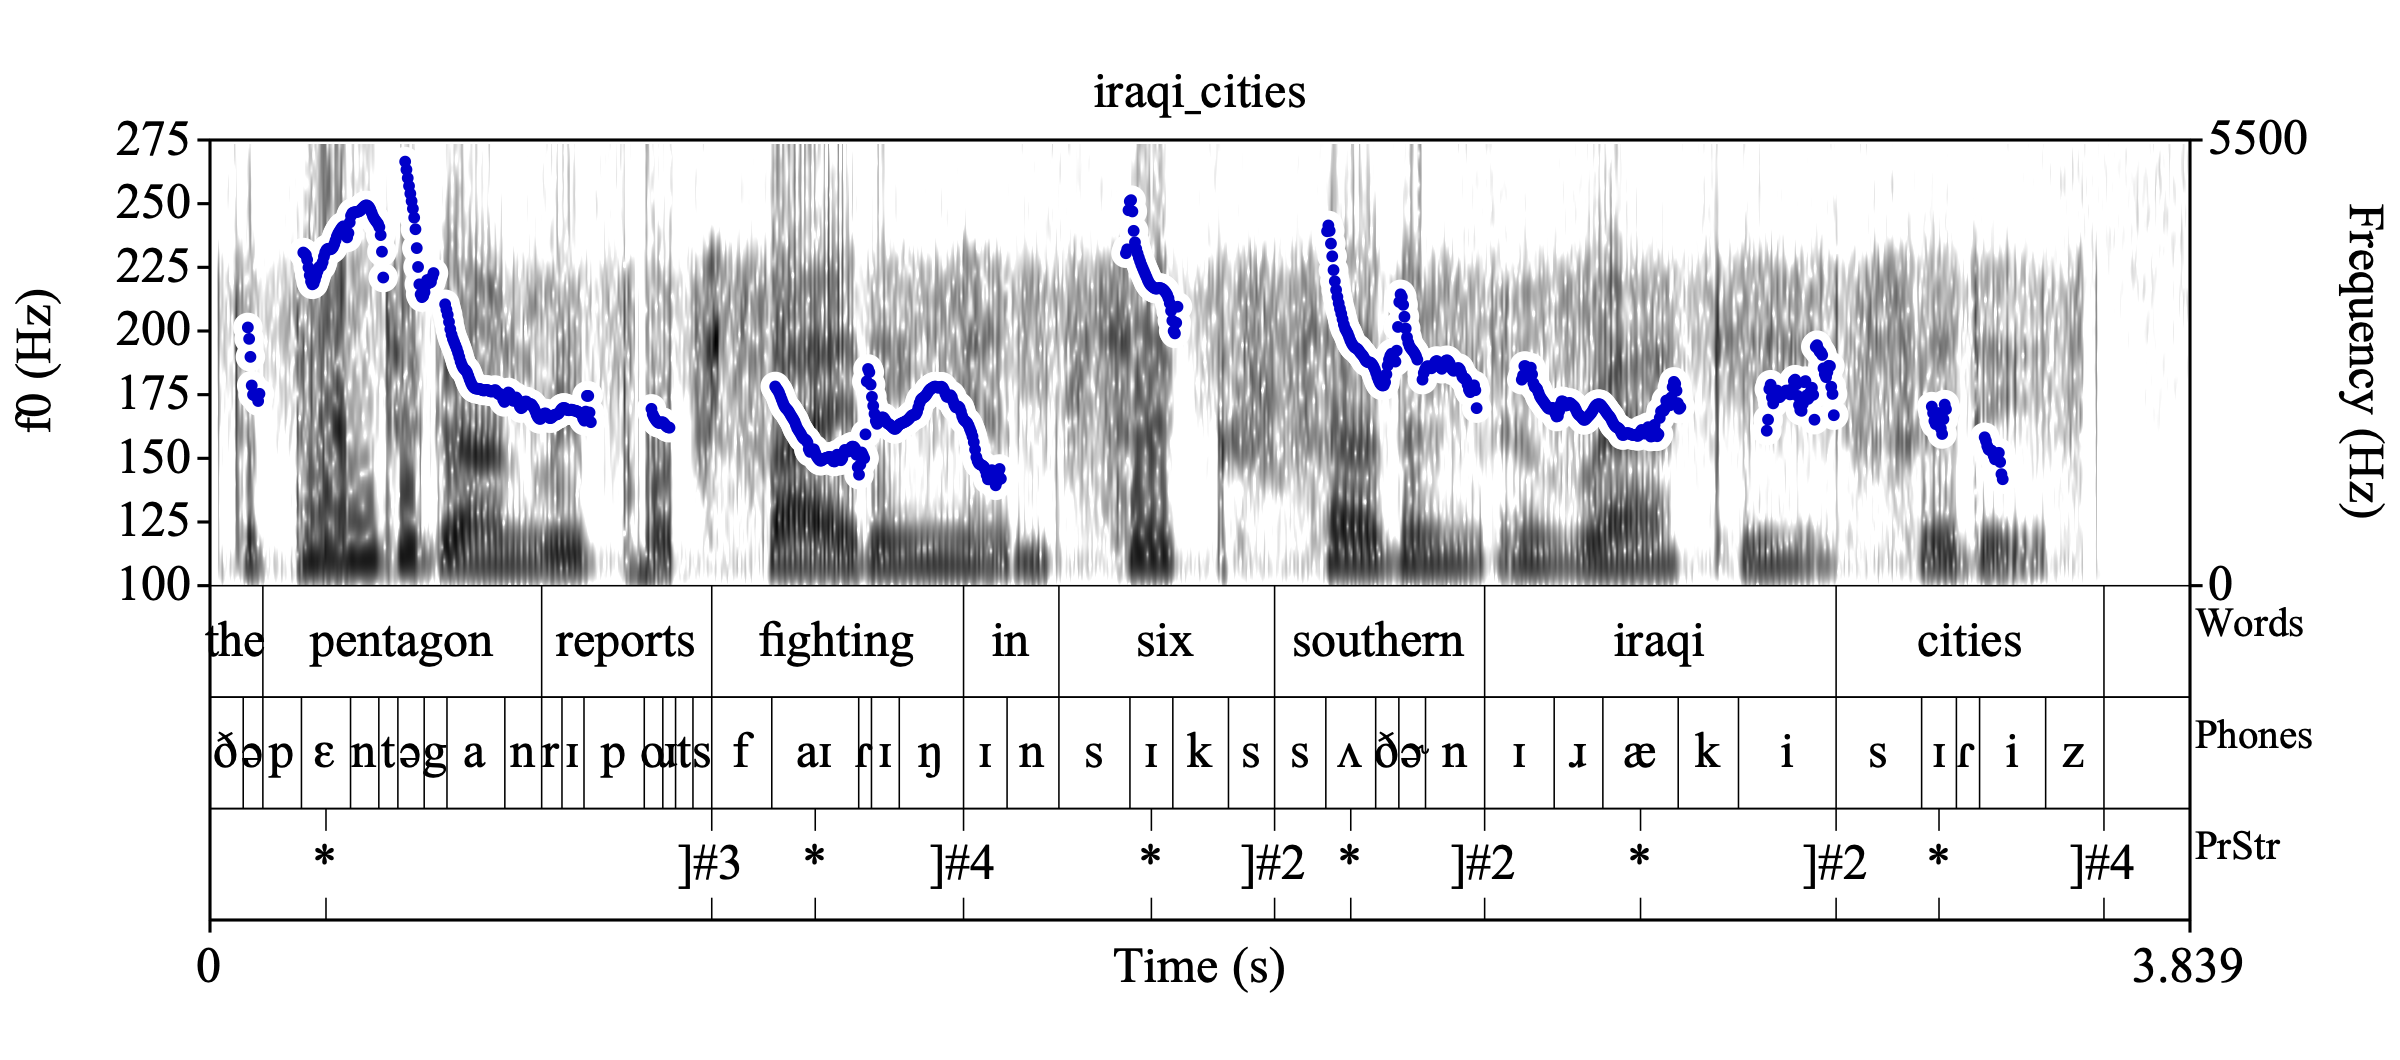
\includegraphics[width=.875\linewidth]{PrStr-iraqi_cities-adv.png}
%
\caption{\texttt{iraqi\_cities}, with analysis tags showing the MAE\_ToBI break indices on the phrase boundary labels.%
\label{fig:iraqi_cities Beyond}%
\index{Annotated example, Beyond the guidelines!iraqi\_cities}
}
\end{figure}

The second example comes from Korean.  In this example, each \textlabel{]} on the PrStr tier is marked with one of the boundary types in the analysis proposed in \citealt{jun07}, including \textlabel{]\#AP}, \textlabel{]\#ip}, and \textlabel{]\#IP}.

\begin{figure}[H]
\centering
%
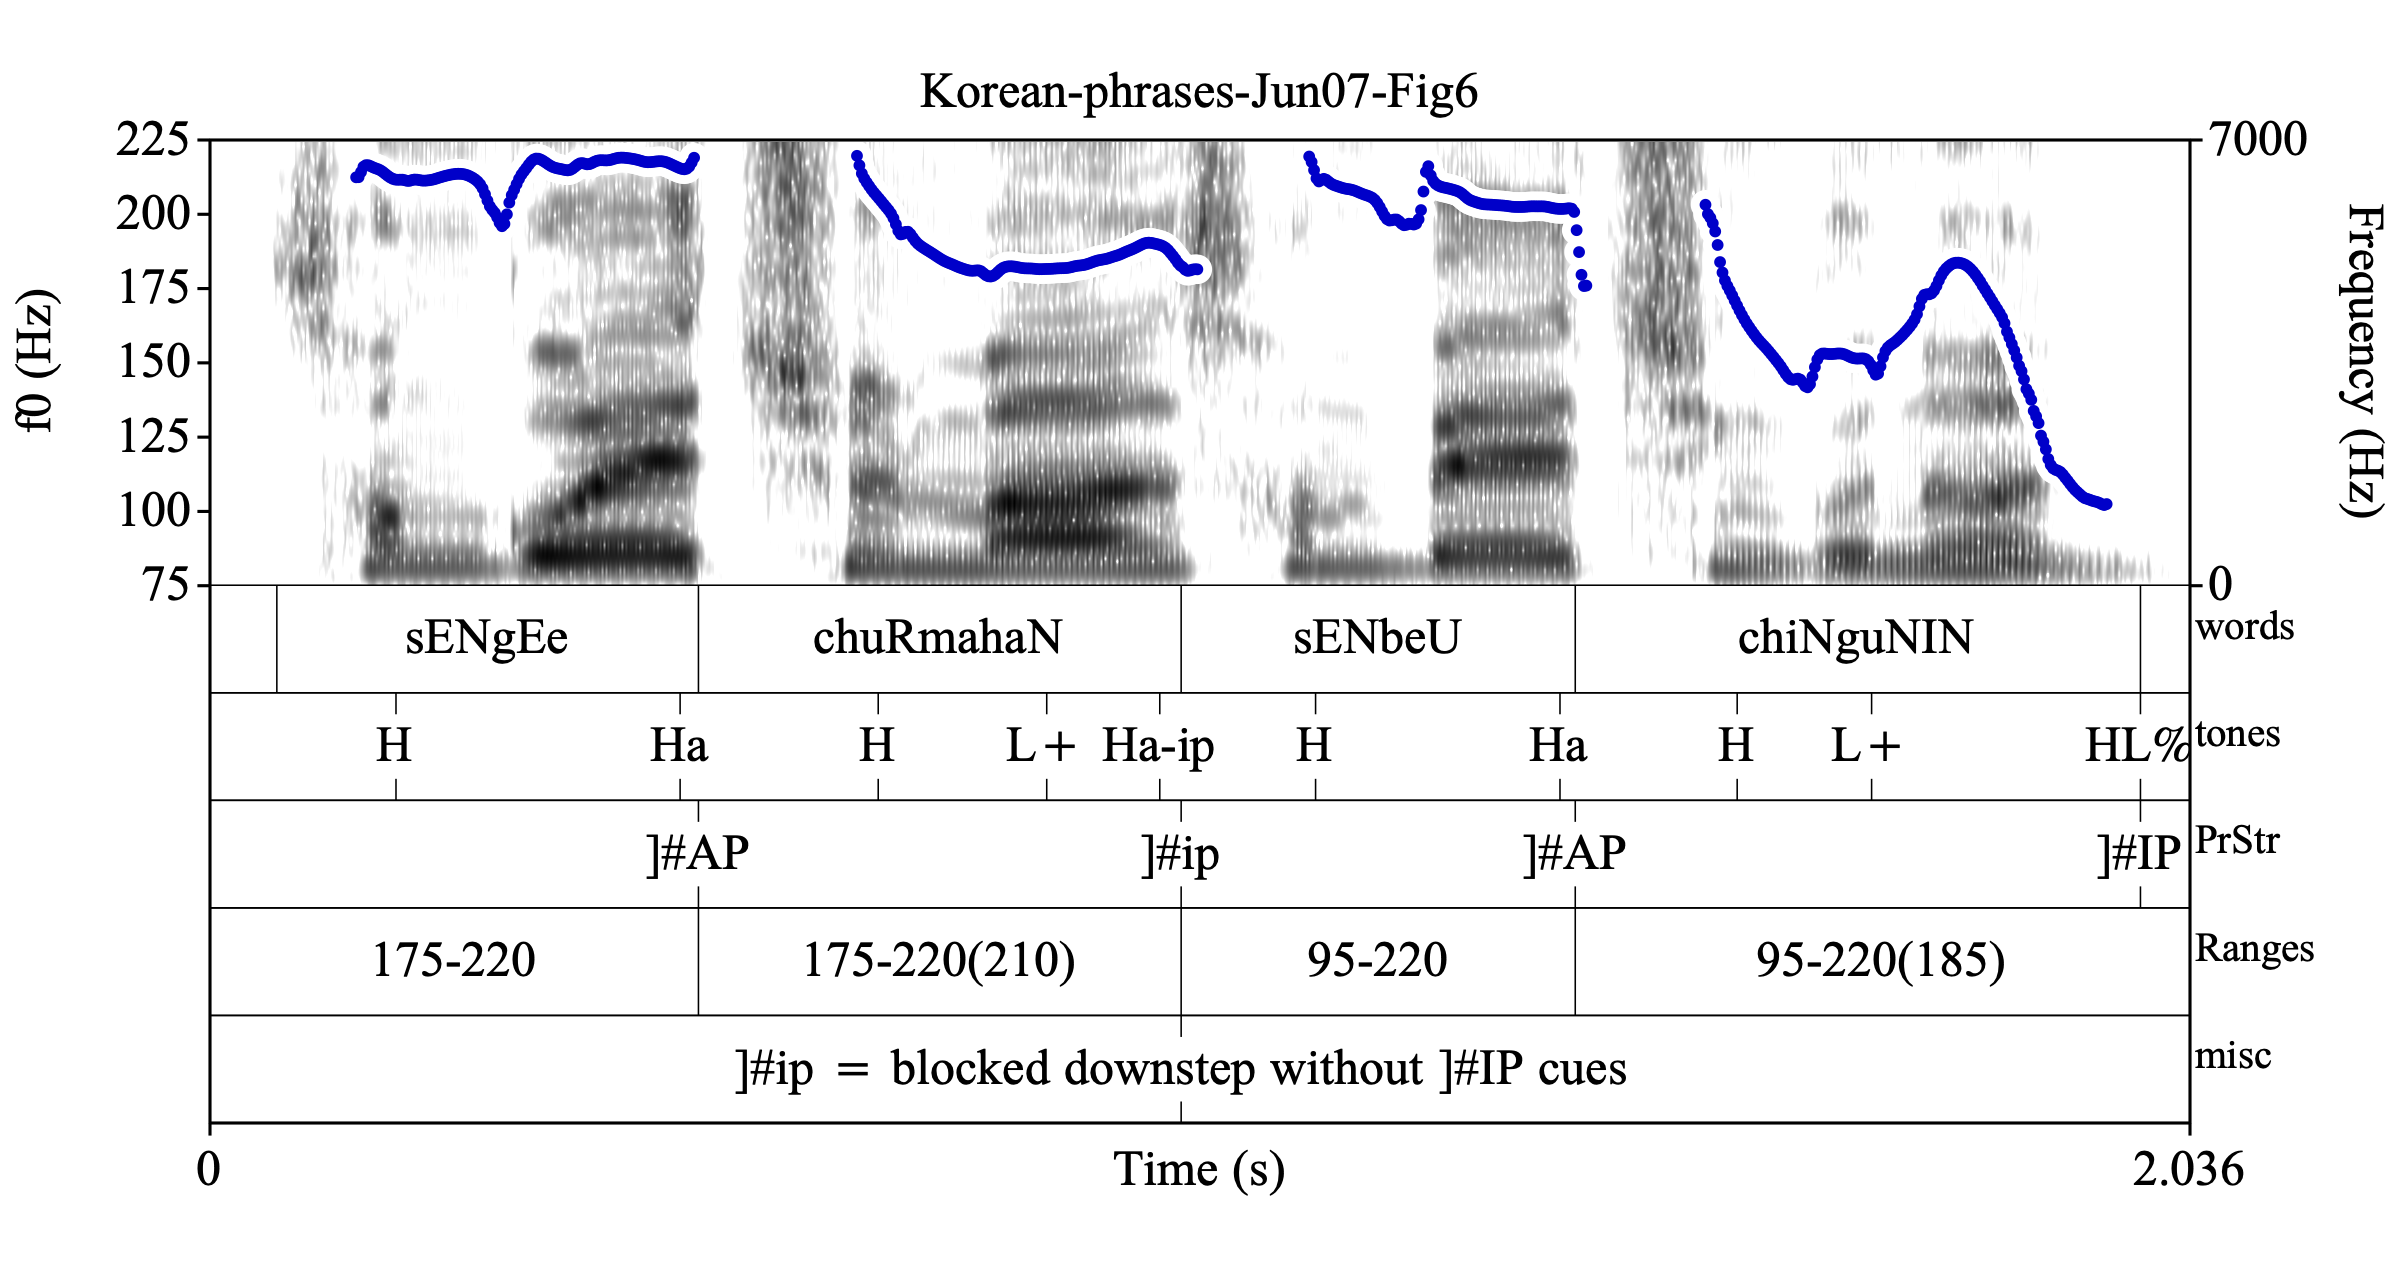
\includegraphics[width=.875\linewidth]{PrStr-Korean-phrases-Jun07-Fig6.png}
%
\caption[\texttt{Korean-phrases-Jun07-Fig6}, with analysis tags.]{\texttt{Korean-phrases-Jun07-Fig6}, with analysis tags showing the proposed addition of ip boundary types to K\_ToBI, as in \citealt{jun07} Fig.6, with PoLaR labels added.%
\label{fig:PrStr-Korean-phrases-Jun07-Fig6}%
\index{Annotated example, Beyond the guidelines!Korean-phrases-Jun07-Fig6}
}
\end{figure}

\subsection{Categories of Phrase-Level Prominence}\label{sec:categories-of-phrase-level-prominence}

The literature on prosodic prominence above the word level has recognized that different strengths of prominence may be linked to different constituents in the prosodic hierarchy. For example, some traditions (e.g., \citealt{libermanprince77}, \citealt{halle-87}, \textit{et seqq}.) state as a principle that in each domain of prosodic hierarchy, the grammar identifies a uniquely prominent element (i.e., “the head”), which often manifests as acoustically\slash perceptually stronger than the other elements. Such analyses predict that each prosodic phrase has a perceptually\slash grammatically “most prominent” element, in addition to the other “prominent” elements. (This approach is directly related to ideas of “nuclear stress” and “nuclear pitch accent”, as well as concepts of “focus stress” and “focus pitch accent”; we return to issues of focus in the next section.)

Given such claims, an advanced labeller may find it useful to identify as many levels of prosodic strength as there are prosodic domains in the prosodic hierarchy. To do so, one can add analysis tags to \textlabel{*} labels, to create PrStr labels like \textlabel{*\#ι} prominences for the strongest \textlabel{*} in an intonation phrase (ι), \textlabel{*\#φ} prominences for the strongest prominence in a phonological phrase (φ), etc., alongside a plain \textlabel{*} for elements that are “prominent” without being most prominent in any particular domain. An example is given below:

\begin{figure}[H]
\centering
%
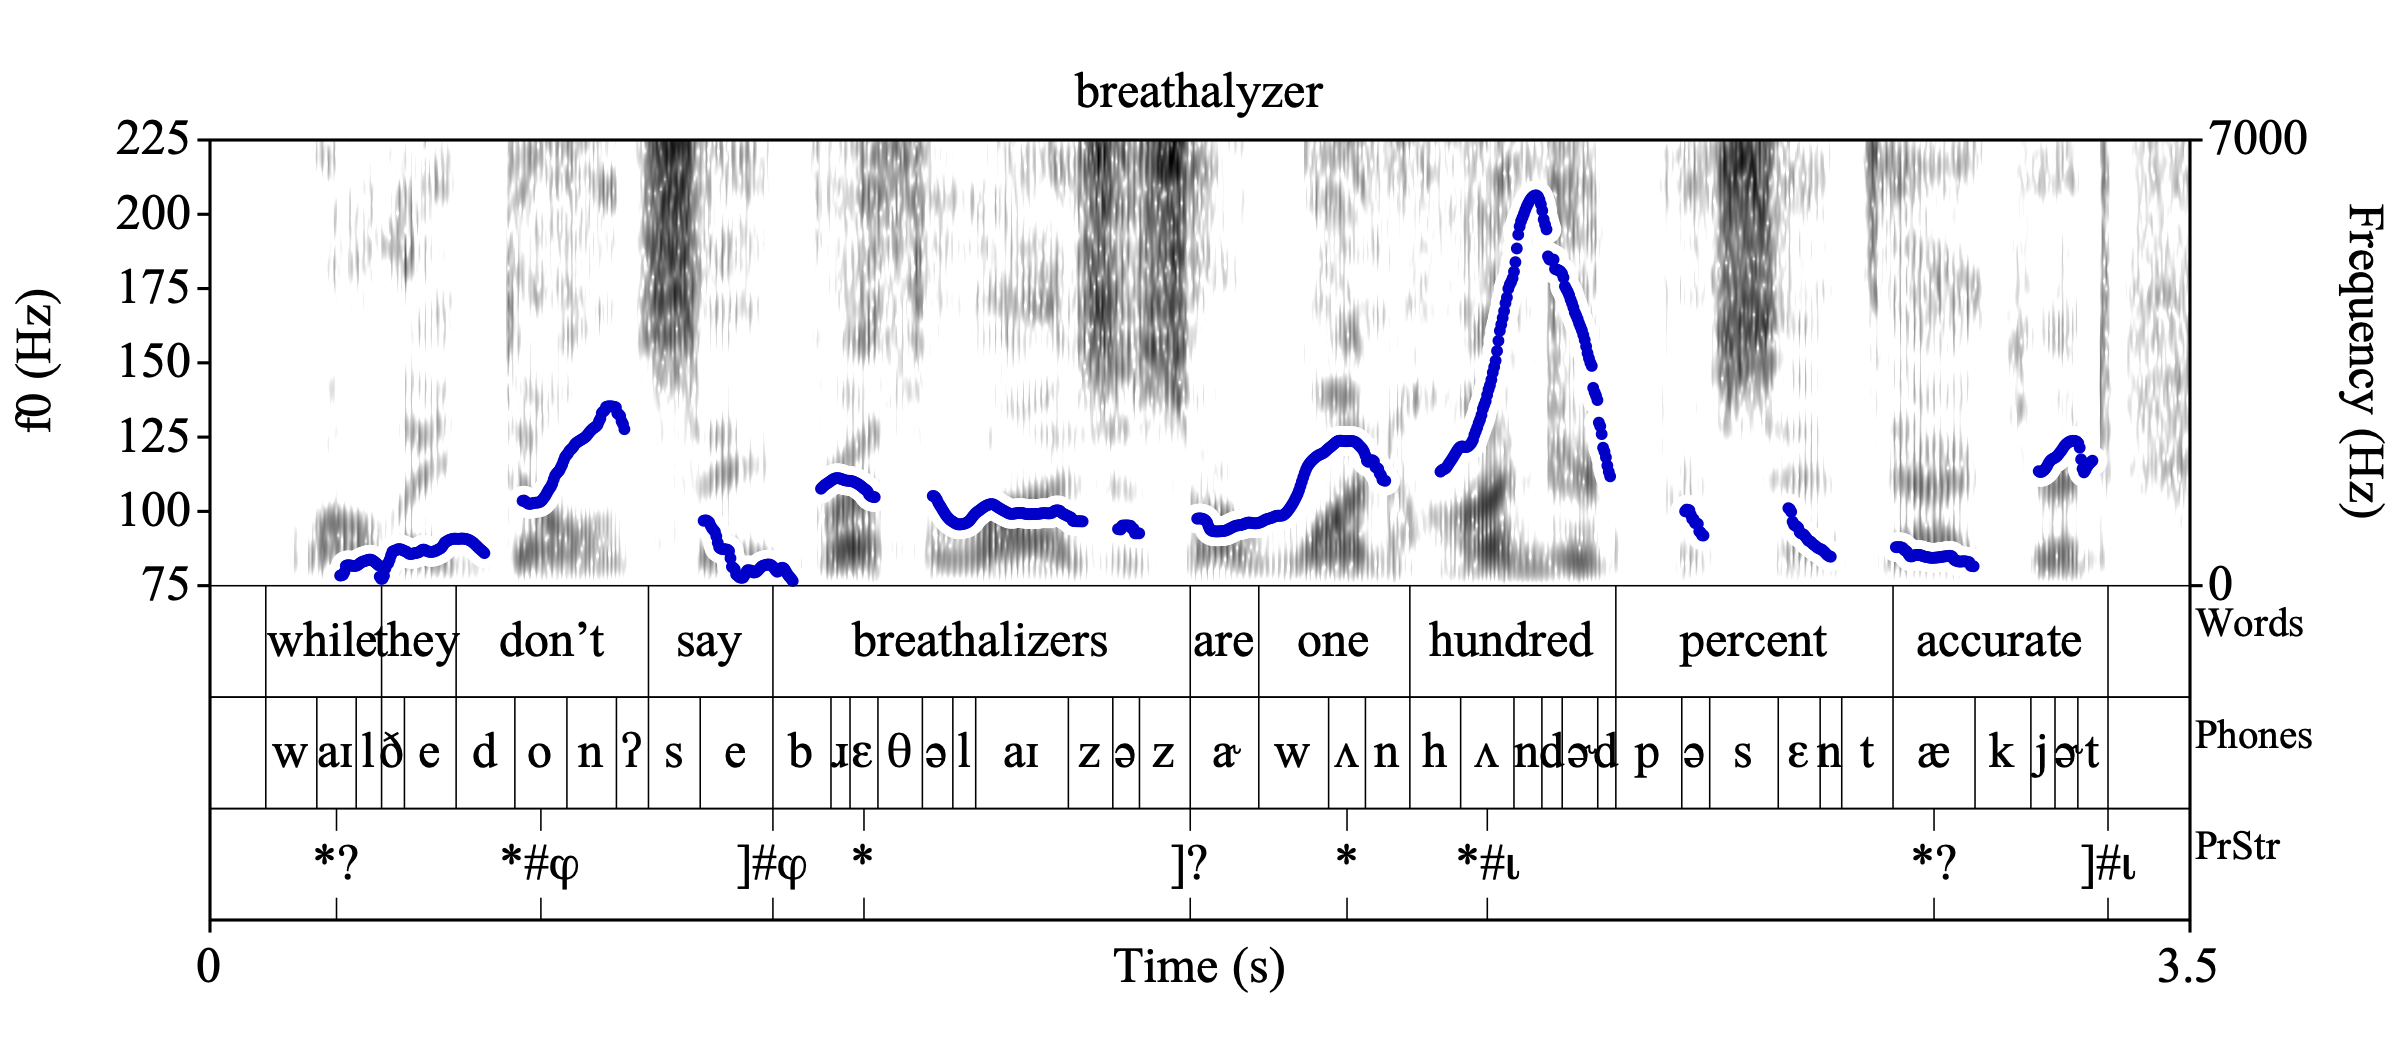
\includegraphics[width=.875\linewidth]{PrStr-breathalyzer-1-adv.png}
%
\caption[\texttt{breathalyzer\_BURNC}, with analysis tags identifying which prominences are strongest in a domain, and which domain each is strongest for.]{\texttt{breathalyzer\_BURNC}, showing the first half of the recording, with analysis tags identifying which prominences are strongest in a domain, and which domain each is strongest for.%
\label{fig:breathalyzer Beyond}%
\index{Annotated example, Beyond the guidelines!breathalyzer}
}
\end{figure}

In this example, the word “\langtext{don’t}” carries the strongest prominence in the phonological phrase “\langtext{while they don’t}”, but “\langtext{hundred}” carries the strongest prominence in the intonation phrase “\langtext{while they don’t say breathalyzers are one hundred percent accurate}”. This sort of grammatical tagging reflects a particular theoretical point of view, and may be subject to a fair amount of disagreement. For this reason, such tags are not a core part of PoLaR. At the same time, PoLaR provides a means for systematically labelling these distinctions, for those who are interested (and who can provide a theoretical stance that allows them to label the proposed  distinctions systematically).

The second half of this sound file illustrates a potential distinction between phonological phrases (φ) and intonational phrases (ι), as well as the most prominent stress in each of these phrasal domains. Labels that reflect this distinction are displayed in Figure \ref{fig:breathalyzer Beyond}.

\begin{figure}[H]
\centering
%
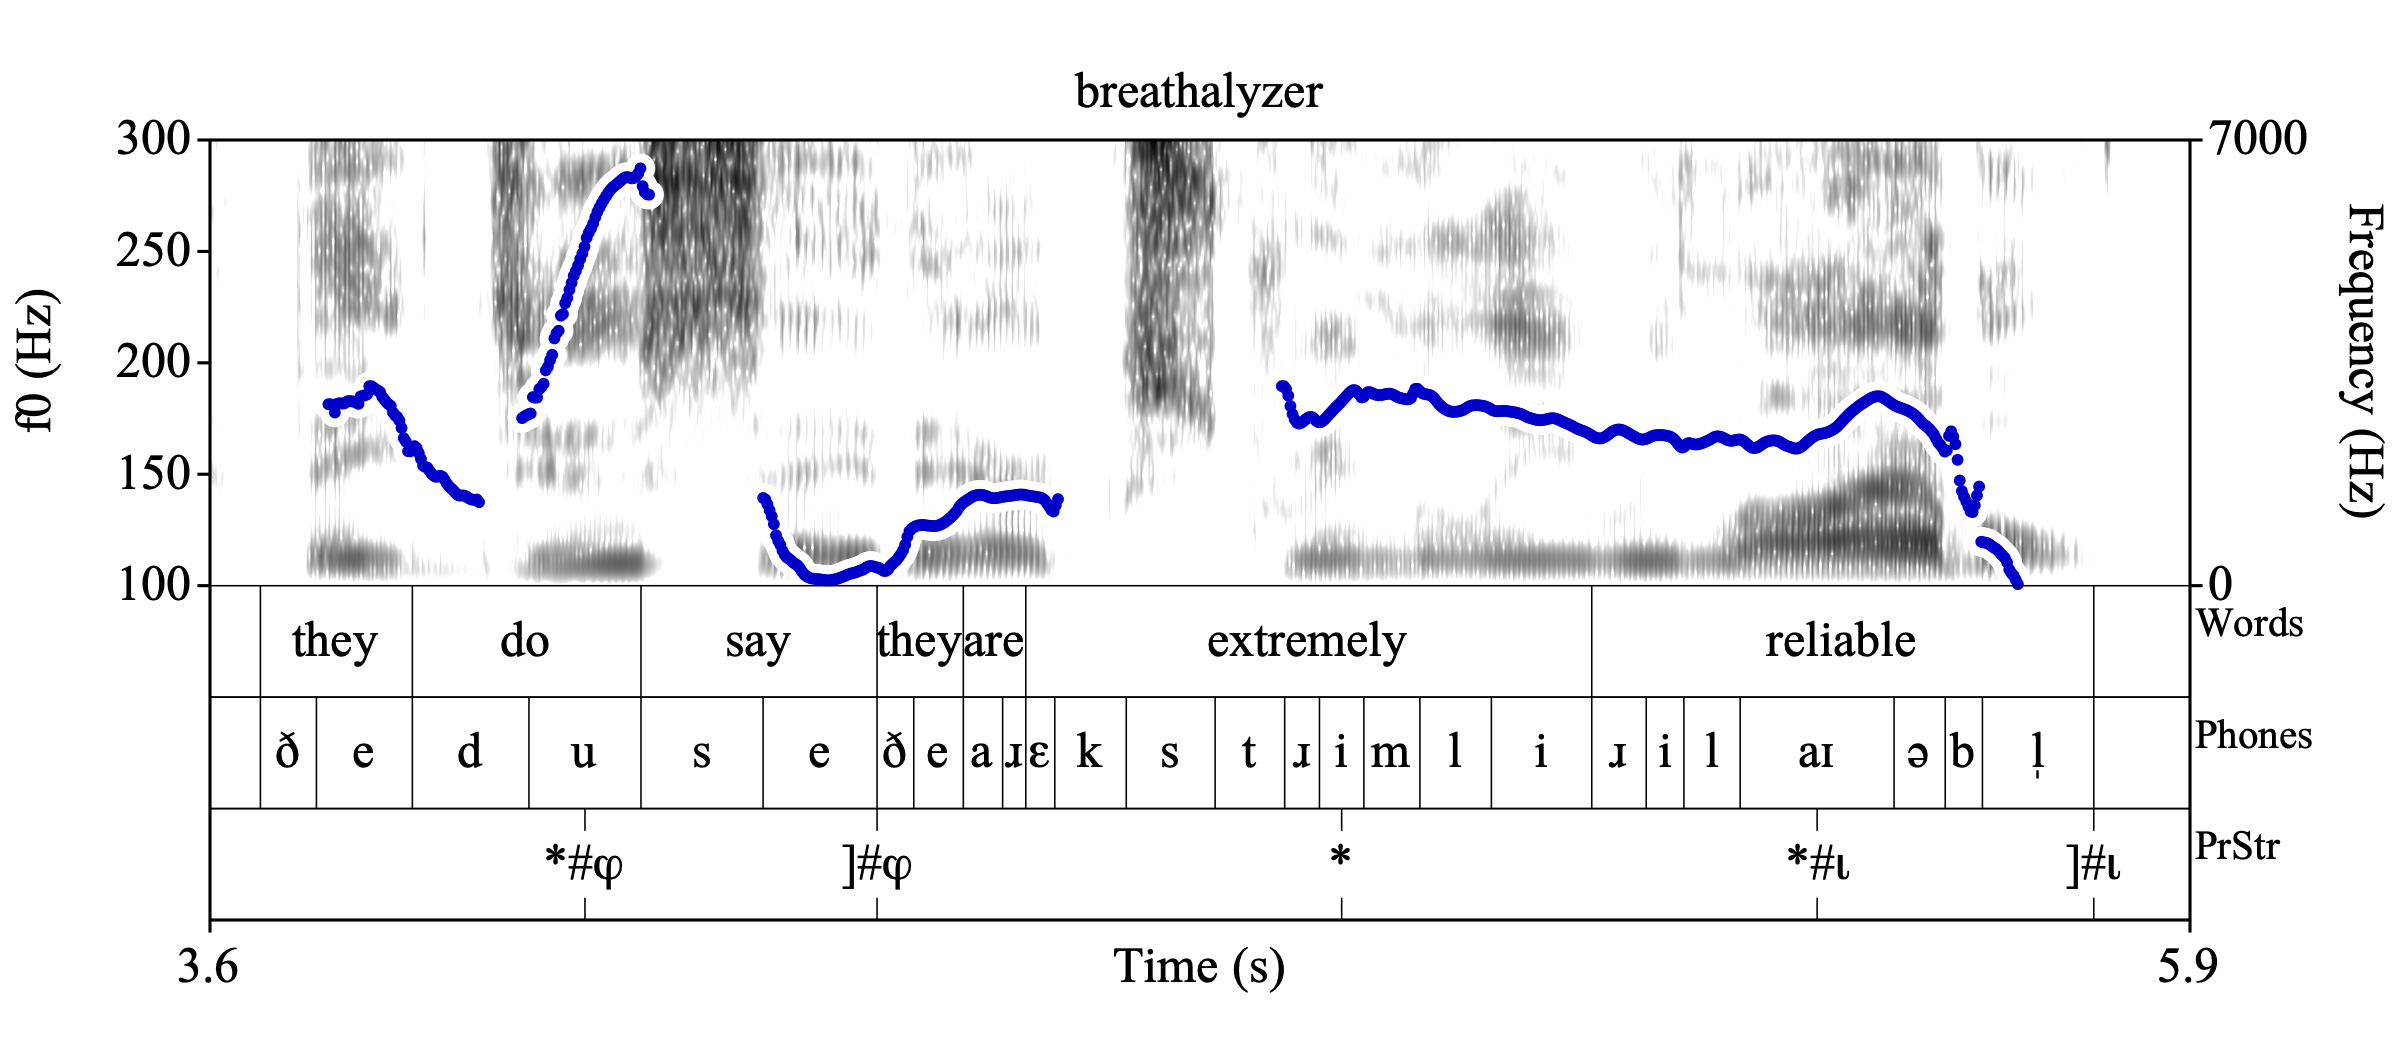
\includegraphics[width=.875\linewidth]{PrStr-breathalyzer-2-adv.png}
%
\caption[The labeller analyzes the first phrase boundary as lower on the hierarchy than the boundary at the end.]{\texttt{breathalyzer\_BURNC}: This is the second half of this recording; the labeller analyzes the first phrase boundary as lower on the hierarchy than the boundary at the end.%
\label{fig:breathalyzer Beyond}%
\index{Annotated example, Beyond the guidelines!breathalyzer}
}
\end{figure}

\subsection{Contrastive Focus Prosody}\label{sec:contrastive-focus-prosody}

In terms of semantic interpretation, contrastive focus is often treated as a grammatical primitive, resulting in the calculation of semantic alternatives (see, e.g., \citealt{rooth92}, \citealt{truckenbrodt95}, \citealt{wagner05}, \citealt{kratzerselkirk20}). In terms of prosody, a variety of languages have been argued to mark contrastively focused elements with particular prosodic forms. For example, contrastive focus may manifest as a particularly strong prominence, which may have a particular intonational form (\citealt{pierrehumberthirschberg90} for American English, \citealt{baltazanijun99} for Greek, etc.) or which may interact in particular ways with surrounding prosodic structure (\citealt{ishihara07} for Japanese, \citealt{kanerva90} for Chichewa, etc.). Taking this idea into account, labellers may wish to systematically label PrStr events with the optional \#CF tag. An English example is provided below.

\begin{figure}[H]
\centering
%
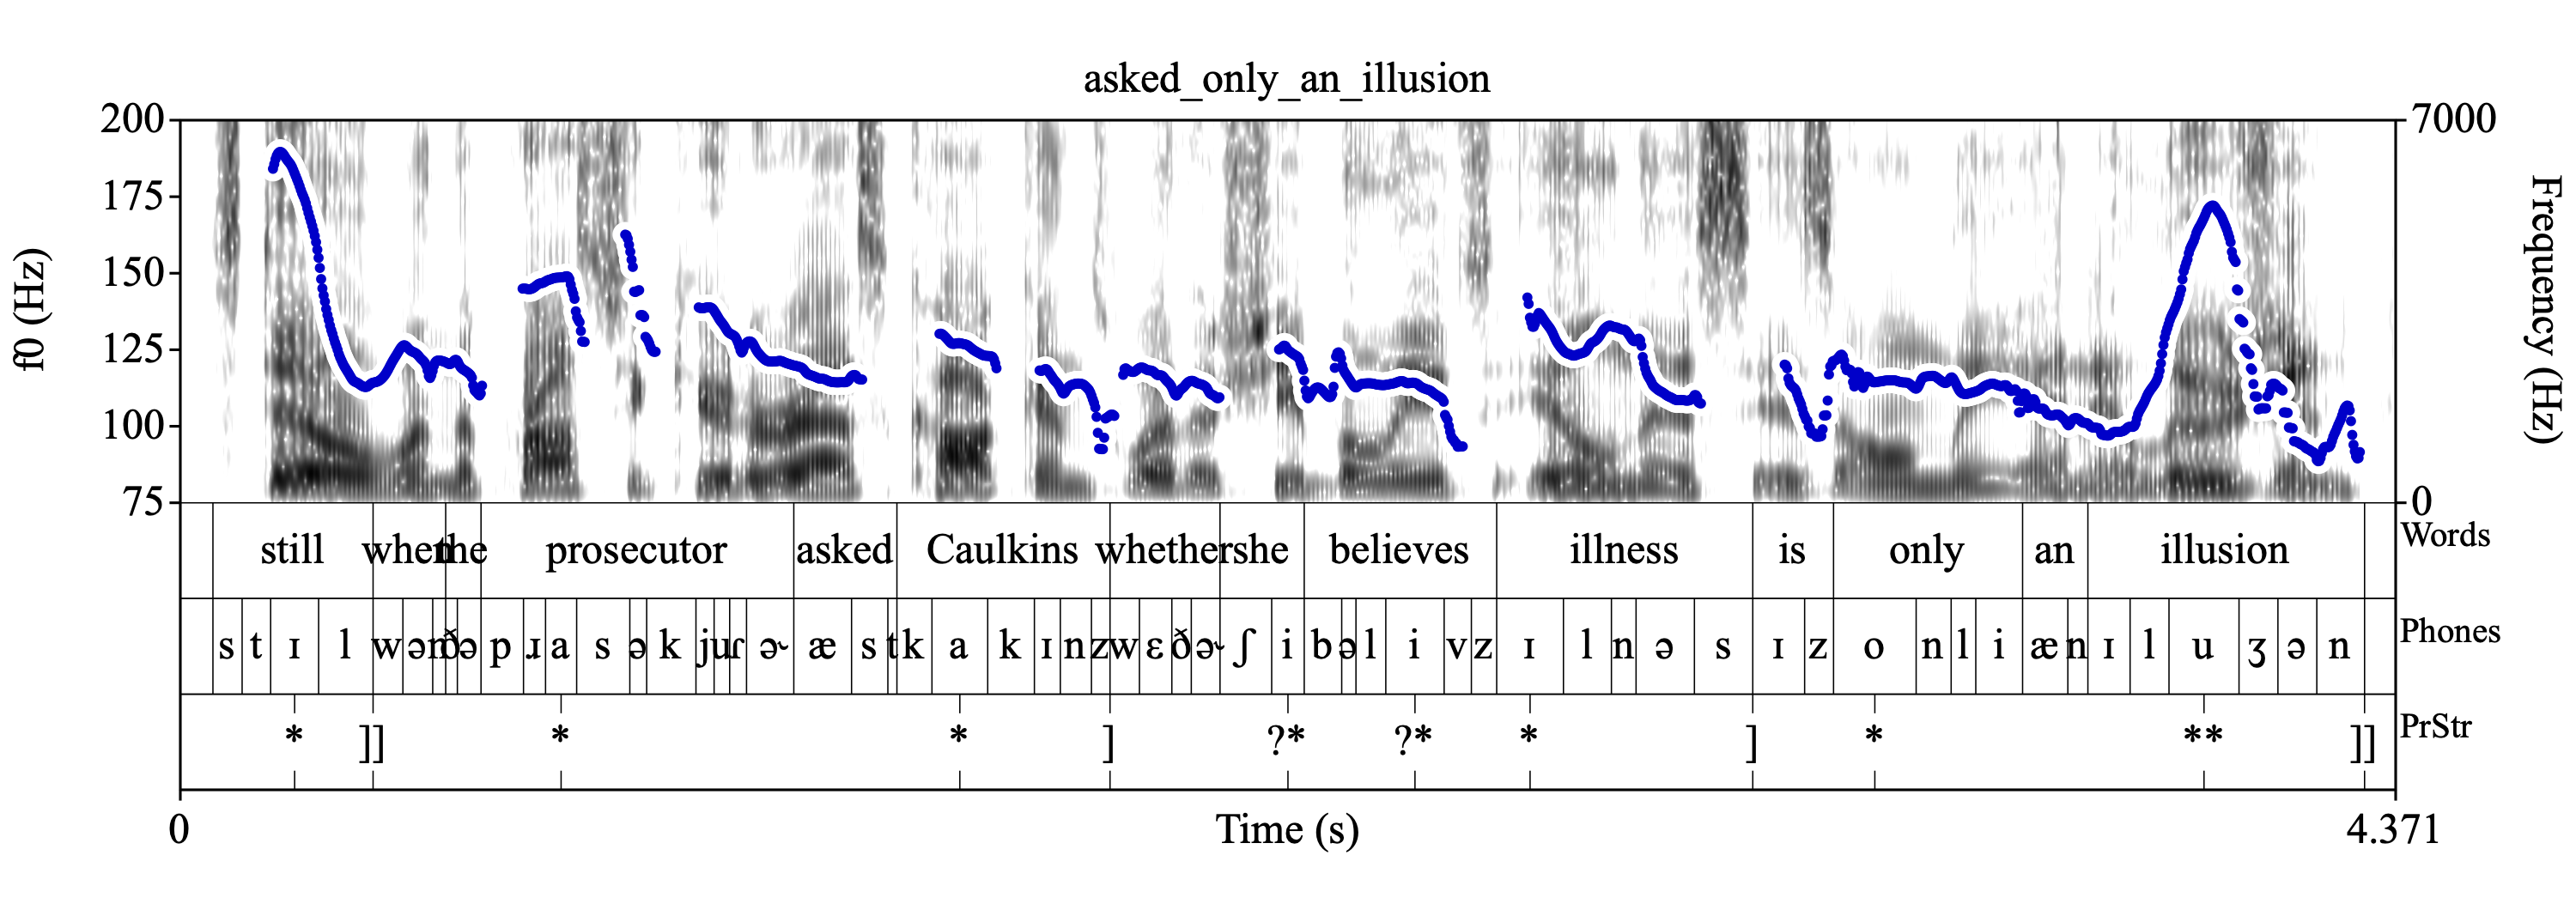
\includegraphics[width=.875\linewidth]{PrStr-asked_only_an_illusion-adv.png}
%
\caption{The labeller has added the ‘analysis tag’ \textlabel{\#CF}, to indicate that the prominence on “illusion” expones the grammatical category of contrastive focus.%
\label{fig:only_an_illusion Beyond}%
\index{Annotated example, Beyond the guidelines!only\_an\_illusion}
}
\end{figure}


Contrastive focus is analyzed as having a grammatical relationship with prominence (and not with phrase boundaries) in English, as the \textlabel{*\#CF} label notates in Figure \ref{fig:only_an_illusion Beyond} above. On the other hand, contrastive focus in other languages is (also) grammatically related to phrase boundaries (e.g., contrastively focused constituents in Korean are marked with an additional phrase boundary; \citealt{jeonnolan17}); in such languages, the \textlabel{\#CF} tag should (also) be added to the appropriate \textlabel{]} or \textlabel{[} label.

\subsection{Summary of Some Proposed Analysis Tags}\label{sec:summary-of-some-proposed-analysis-tags}

We have reviewed some examples of potential \#X t tags as a way of annotating grammatical analyses made by the labeller. Some of the types of tags discussed here are listed in Table \ref{tab:beyond polar tags}.

\begin{longtable}{cp{.3\linewidth}p{.5\linewidth}}
\toprule \textbf{Label} & \textbf{Phonological Object} & \textbf{Time-Aligned with} \tabularnewline
\midrule
\endhead
\textlabel{]\#X} & Phrase Boundary for a Phrase of Type “X” & A prosodic phrase ends at this point; the type of prosodic phrase is specified by “X” (e.g., \textlabel{]\#IP}) \tabularnewline\hdashline
\textlabel{[\#X} & Phrase Boundary for a Phrase of Type “X” & A prosodic phrase begins at this point; the type of prosodic phrase is specified by “X” (e.g., \textlabel{[\#IP}) \tabularnewline\hdashline
\textlabel{*\#X} & Strongest Prominence in a Domain & The constituent this occurs in is the most prominent in the prosodic domain specified by “X” (e.g., \textlabel{*\#IP}) \tabularnewline\hdashline
\textlabel{*\#CF} & Contrastive Focus Prominence & The prominence marks Contrastive Focus meaning \tabularnewline
 \bottomrule 
\caption{A summary of some of the analysis tags described in this section, as expert-level PrStr annotation.}
\label{tab:beyond polar tags}
\end{longtable}

The goal of including these examples here is to show how an annotator can use tags to systematically notate their theoretical analyses. PoLaR annotators are strongly encouraged to devise their own tags; when doing so, they should explicitly define the grammatical features that each tag marks, and provide guidelines on when it should (or should not) be used. Analysis tags thus provide PoLaR with flexibility, so that it can be used for systematic purposes not foreseen by these guidelines.

\section{Adding a New Tier}\label{sec:adding-a-new-tier}

PoLaR is meant to be extensible and new Tiers may be added to address particular research questions. New tiers can always be added without serious consequence for the existing tiers and their labels, because the tiers are designed to, by default, isolate particular characteristics of the speech signal. These Tiers can be shared with the community by sending  supporting material to the authors for inclusion on \href{https://www.polarlabels.com}{polarlabels.com}. This repository can also be referenced in publications if useful. 
 
There are several issues, both theoretical and practical, to consider when developing a new Tier. First, one should consider whether the new Tier is necessary or whether additional labels on existing tiers would suffice. Second, labels should be unique,  memorable and consistent. Finally, labels should be machine readable. 

Supporting materials should include:
\begin{enumerate}
	\item a README.txt text  file that includes
	\begin{enumerate}
		\item the date and version number (e.g. 1.0) 
		\item a brief description of the motivation, structure  and use of the new Tier’s labels. This README can also include labelling guidelines.
		\item bibliography and reference materials for the phenomenon to be labelled
		\item a summary table of the labels (formatted like Table XX and others in this guide)
	\end{enumerate}
	\item sound and Textgrid file(s) for a labelled example (or several, to illustrate contrastive phenomena),
	\item any scripts that would be helpful in labelling. 
\end{enumerate}

\subsection{New Tier Candidate: Labelling Individual Cues to Prosodic Structure}\label{sec:labelling-individual-cues}
At the heart of PoLaR’s approach to labelling prosody is a focus on cues in the intonational domain that involve f0 patterns.  But as has often been noted in this monograph, speakers use many other cues to signal both prominence and grouping, and to signal other aspects of meaning such as emotion, attitude, and stance. As noted earlier, the range of cues in the speaker’s toolbox includes patterns of duration, amplitude and voice quality, in addition to f0, and it has been argued that changes in the cues to the distinctive features of the phonemes of a word can also serve as cues to prosodic structure. It is thus of considerable interest to some researchers to understand how speakers (and listeners) use the different individual cues available to them.  \citet{brugos-18}, for example, have shown that a location that is marked by more cues (e.g. f0 movement at the end of a word, f0 reset at the beginning of a word, amplitude changes, final creak at the end of a phrase, irregular pitch periods at the onset of a phrase, pause and final lengthening) is more likely to be labelled as a boundary by ToBI labellers.  They have also argued that different listeners may weight each cue type differently in perception. PoLaR’s flexible extensibility facilitates investigation of such ideas, by allowing labellers to develop tiers and conventions for annotating individual cues separately. 

Taking the broader view,  the expansion of labelling systems to include individual acoustic cues is also occurring in the domain of cues to the distinctive features that define natural classes of phonemes.  For example, \citet{stevens02} proposed that listeners attend to Landmark cues (i.e. moments of abrupt change in the spectrum of the wave form, associated with narrowings and widenings of the vocal tract) and other acoustic cues to feature contrasts in a spoken utterance.  Relatedly, \citet{stevenskeyser89} and \citet{keyserstevens01} proposed that speakers can enhance a contrast either phonologically, by adding an enhancing feature (e.g. [+round] for /ʃ/ in American English), or phonetically, by adding an enhancing cue (e.g. vowel shortening before a voiceless coda in American English).  (See \citealt{clements09} for further discussion.)   In this sense, PoLaR offers the opportunity not only to extend prosodic labelling to individual cues, but also to integrate prosodic cue labelling with distinctive feature cue labelling in the segmental domain.  This integration would provide a powerful tool for quantifying the interaction between prosodic structure and systematic variation in segmental feature cues, and investigating the principles and constraints that govern this interaction.  

\subsection{New Tier Candidate: Analyzing Range Changes}\label{sec:new-tier-range-changes}
The selection of pitch range(s) for an utterance has been associated with a variety of linguistic functions, communicative\slash emotional signalling, and paralinguistic phenomena. In the Basic and Advanced Ranges chapters above, we have described and given examples for a number of phenomena in which range changes are frequently observed.  While we have offered guidance about how to determine where to put range boundaries and choose range values, this guidance is somewhat agnostic about the reasons why range changes occur. In other words, the Ranges tier labels capture what the values of the ranges are, but do not specify why range changes occur. 

Much like the way in which the Advanced Points tier labels associate\slash assign individual turning points to PrStr tier objects (prominences and boundaries), we envision that researchers may want to link range changes to aspects of prosodic structure, or even discourse or syntactic structure. We encourage researchers to develop annotation schemes for such links that are consistent with PoLaR conventions. Such annotations might include, for example, elements like associating a Ranges tier annotation with a PrStr element (i.e. \textlabel{*}, \textlabel{[}, or \textlabel{]}) as well as additional expansions. While future developments may incorporate additional labels in the Ranges tier itself, we encourage researchers to consider making use of a new tier for such ‘linking labels’. As in any expansion to PoLaR, it is critical that the researchers proposing the expansion provide a clear set of guidelines, to explain and describe such new tiers and/or labels.

Conventions laid out in §\ref{sec:points-advanced} for the Advanced Points tier labelling (namely, association between PrStr objects and f0 points) incorporate insights based on theories accounting for intonational movements that are well-established in the intonational phonology literature. Associations between pitch ranges (sometimes called registers) and prosodic structure are less firmly established in the same literature. That being said, the flexibility of PoLaR’s tier-based annotation system encourages the use of annotations to explore hypotheses about associations between ranges and aspects of prosodic structure, facilitating potential future studies in this domain. 

\textbf{Examples of changes to ranges that may be governed by prosodic structure and discourse structure:}
\begin{itemize}
	\item Range maximum is conditioned by a compression relating to a sequence of prominences (i.e. frequently considered a “downstepped” High pitch accent) 
	\begin{itemize}
		\item This may include cross-phrase pitch-accent scaling relations (\citealt{fery-05}), an issue that is in need of study, since current AM theory (and the ToBI annotation system) provides for downstep only within an intonational phrase. 
	\end{itemize}
	\item Range maximum is conditioned by an expansion relating to a sequence of prominences (i.e. sometimes considered an “upstepped” High pitch accent) 
	\item Range (max and/or min) is conditioned by phrase boundaries or higher level grouping, including:
	\begin{itemize}
		\item parentheticals
		\item embedded registers (\citealt{truckenbrodt02}; \citealt{dimperio-10})
		\item long-distance range dependencies (\citealt{ladd88})
		\item larger discourse structure (including what has been called “paragraph intonation”) (\citealt{lehiste75}, \citealt{sluijter-93}, \citealt{wichmann14})
	\end{itemize}
\end{itemize}

As our understanding of such phenomena deepens, and testable hypotheses emerge, PoLaR’s ability to expand by adding new tiers and connecting information across tiers will prove useful.


\bibliographystyle{glossa.bst}
\bibliography{localbibliography.bib}

\end{document}	